\section{K-Nearest Neighbors Classification}
\begin{multicols}{2}

Now that we've gotten a sense for what's in our data set, as a simple example to get started, we're going to use this data set to train a classifier that will automatically identify any future pieces of fruit that might come our way. Based on the features available to the classifier such as the object's color, size and mass. To do this, we'll use a popular and easy to understand type of machine learning algorithm known as \emph{k-nearest neighbors} (k-NN). 

The \texttt{K-Nearest Neighbors} algorithm can be used for \emph{classification} and \emph{regression}. Though, here we'll focus for the time being on using it for classification. 

\texttt{k-NN} classifiers are an example of what's called \emph{instance based or memory based supervised learning}. What this means is that instance based learning methods work by \emph{memorizing} the labeled examples that they see in the training set. And then they use those memorized examples to classify new objects later. 

The \textbf{\texttt{k}} in \texttt{k-NN} refers to the number of nearest neighbors the classifier will retrieve and use in order to make its prediction. 

In particular, the \texttt{k-NN}  algorithm has three steps:

First of all, when given a new previously unseen instance of something to classify, a k-NN classifier will look into its set of memorized training examples to find the k examples that have \emph{closest features}. 

Second, the classifier will look up the \emph{class labels} for those k-Nearest Neighbor examples. 

And then once it's done that, it will \emph{combine} the labels of those examples to make a prediction for the label of the new object. Typically, for example, by using simple \emph{majority vote}. 

Let's look at a visual example of a k-NN classifier that is based on our fruit data set. 

So what I've done here is taken our training set and plotted each piece of fruit using two of its features. The width and the height. 

These two features together form what is called the feature space of the classifier. 

And I've shown each data point's label using the colors shown in the legend. So as you can see, there are four different colors here that correspond to the four types of fruit that are in our data set. 

\begin{center}
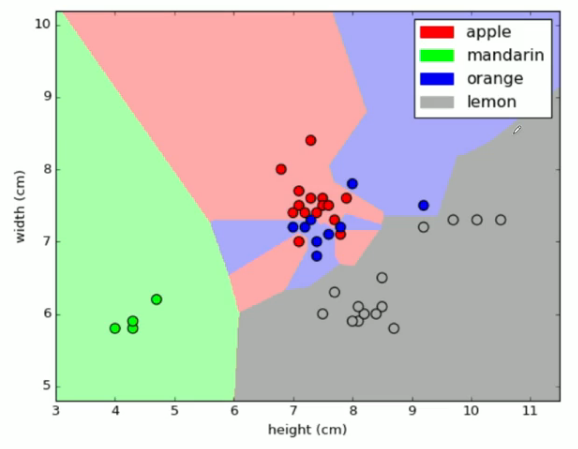
\includegraphics[width=\linewidth]{img/kNN-Classifier-k1-example.png}
\end{center}

These broad areas of color show how any point, given a width and height, could be classified according to a one nearest neighbor rule. So, in other words, I've set k = 1 here. So, for example, a data point over here that had a height of six centimeters and a width of nine centimeters would be classified as an apple. Because it falls within this red area here that the k-NN classifier has decided map two objects that are apples based on the dimensions. Or for example if I saw that the classifier saw a piece of fruit that had a height of four centimeters and a width of seven centimeters, it would be classified as a mandarin orange. Because it falls within this decision area that's assigned to mandarin oranges. 

So what does it mean to have a one nearest neighbor rule? Where did it come up with these different class assignments in the first place? 

Well, let's take a look at the apple example over here. 

The object that has a height of six centimeters and a width of nine centimeters, if you give the classifier that point, what it will do is search within all the different training examples that it's seen. So it would look at all these points and see which one is closest, so we're looking at the nearest single neighbor. So we're looking at k=1. We're trying to find the one point that's closest to our, what's called the query point. This is the point we want to classify. 

So, in this case, we can see probably that this point over here is the nearest neighbor of the query point in feature space. Similarly, if we look at the mandarin example over here, 

the closest training set object to the query point is one of these probably, maybe this point right here. Okay, so that's the nearest neighbor of that query point. 

So for any query point in the future space, let's say we're over here in the lemon zone. The nearest neighbor to this query point would be this training set point right here. 

And because the training set points are labeled, we have the labels for those, in the one nearest neighbor case, the classifier will simply assign to the query point, the class of the nearest neighbor object. 

Because the nearest neighbor here is an apple, 

the query point here will get classified as an apple. If we look at the mandarin orange point over here, the nearest data point is the mandarin orange. So it will get classified in that region. And if we do that for every possible query point, we get this pattern of class regions. The zones where we transition from one class to another, this line right here is called the decision boundary. Because query points that are on one side of the line get mapped to one class. And points that are on the other side of the line get mapped to a different class. 

So, because this is a k-nearest neighbor classifier, and we are looking at the case where k = 1, we can see that the class boundaries here, the decision boundaries. Let's take an example over here. We have a point over here that's an orange, another point that's a lemon here. And we can see the decision boundary because it's based on Euclidean distance and we're weighting points equally that the decision boundary goes exactly at a distance equidistant to these two things. That's exactly halfway between these two points, right? Because if it were any closer to this point, it would be mapped to the orange class. And if it were any closer to the lemon instance over here, it would be mapped as lemon class. So you can see this pattern for all the decision boundaries here. This line is equidistant to these two nearest points. 

So this is basically how the K-Nearest Neighbor classifies new instances. So you can imagine with query points where k is larger than 1, we might use a slightly more complicated decision rule. Let's take this example over here. Suppose we have a query point that's in orange. And we're doing two nearest neighbours classifications. So in that case, the two nearest points are these two points here. And in cases where k is bigger than 1, we use a simple majority vote. We take the class that's most predominant in the labels of the neighbor examples. So in this case, the labels happen to agree they're both oranges. And so this point in a two nearest neighbors situation would be classified as an orange. 

When you get points that are closer to, say, a point over here, the two nearest neighbors, in that case, might be these points here. 

In which case you could choose randomly between them to break the tie. Typically, the value of k is odd, so that we can simply, k equals three it might look like this. And so, you can see that the three nearest neighbors here are a red point an apple, a blue point an orange, and another red point an apple. So, in the k = 3 case, the vote would go towards labeling this as an apple. 

And that's basically all there is to the basic mechanism for k-NN classifiers. 

\subsection{Parameters}

More generally, to use the nearest neighbor algorithm, we specify four things:

\begin{enumerate}

\item define what \emph{distance} means in our future space, so we know how to properly select the nearby neighbors. In the example that I just showed you with the fruit data set, we used the simple straight line, or euclidean distance to measure the distance between points. 

\item we must tell the algorithm \emph{how many} of these nearest neighbors to use in making a prediction. This must be a number that is at least one. 

\item we may want to give some neighbors more influence on the outcome. For example, we may decide that neighbors that are closer to the new instance that we're trying to classify, should have more influence, or more votes on the final label. 

\item once we have the labels of the k nearby points, we must specify how to combine labels to produce a final prediction. 
\end{enumerate}

Here's a specific example of some typical choices we might make for these four things. 

The most common distance metric and the one that scikit-learn uses by \textbf{default} is the \texttt{Euclidean no straight line} distance. 

So, technically if you are interested, the Euclidean metric is actually a special case of a more general metric called the \texttt{Minkowski} metric, where there is a parameter \texttt{p~=~2} that will give you the Euclidean metric. 

We might choose to use the five nearest neighbors, let's say, for our choice of k. 

And, we might specify that there's no special treatment for neighbors that are closer, so we have a \texttt{uniform} weighting. 

Also by \textbf{default} scikit-learn will apply for the fourth criterion a \emph{simple majority vote}, and it will predict the class with the most representatives among the nearest neighbors. 


For now, let's take a look at the notebook to see how we apply a k nearest neighbor classifier in Python to our example fruit data set. 

{\scriptsize
\begin{verbatim}
from sklearn.neighbors import KNeighborsClassifier

knn = KNeighborsClassifier(n_neighbors = 5)
knn.fit(X_train, y_train)
KNeighborsClassifier(algorithm='auto', leaf_size=30, 
   metric='minkowski', metric_params=None, n_jobs=1, 
   n_neighbors=5, p=2, weights='uniform')

knn.score(X_test, y_test)
0.53333333333333333           
\end{verbatim}
}

Our task was to correctly classify new, incoming objects. In our example case, pieces of fruit. So, our newly trained classifier will take a data instance as input, and give us a predicted label as output. 

Now, what I'm doing next here in the notebook is defining a dictionary that takes a numeric fruit label as the input key. And returns a value that's a string with the name of the fruit, and this dictionary just makes it easier to convert the output of a classifier prediction to something a person can more easily interpret, the name of a fruit in this case. 

So, for this example we'll define a variable \texttt{X} that holds the features of our data set without the label. And here I 'm going to use the mass, width and height of the fruit as features. So, this collection of features is called the \emph{feature space}. 

We define a second variable \texttt{y} to hold the corresponding labels for the instances in \texttt{X}. 

Now, we can parse \texttt{X} and \texttt{y} to the \texttt{train_test_split} function. Normally these splitting into training and test sets is done randomly, but for this lecture I want to make sure we all get the same results. So, I set the \texttt{random_state} parameter to a specific value, in this case I happen to choose~\texttt{0}. 

The results of the train test split function are put into the four variables you see on the left. And these are marked as x_train, x_test, y_train, and y_test. We're going to be using this x and y variable naming convention throughout the course to refer to data and labels. 

Once we have our train-test split, we then need to create an instance of the classifier object. And in this case a k-NN classifier. 

And the set the important parameter in this case the number of neighbors to a specific value to be used by the classifier. 

We then train the classifier by passing in the training set date in X_train, and the labels in y_train to the classifiers fit method. 

Now, the k-NN classifier that I'm using in this case is an example of a more general class called an estimator in scikit-learn. So, all estimators have a fit method that takes the training data, and then changes the state of the classifier, or estimator object 

to essentially enable prediction once the training is finished. 

In other words it updates the state of the k and n variable here, which means, that in the case of k-nners neighbors it will memorize the training set examples in some kind of internal storage for future use. 

And that's really all there is to training the k-NN classifier, and the first thing we can do with this newly trained classifier is to see how accurate it's likely to be on some new, previously unseen instances. 

To do this, we can apply they classifier to all the instanced in the test set that we've put aside. Since these test instances were not explicitly included in the classifiers training. 

One simple way to assess if the classifier is likely to be good at predicting the label of future, previously unseen data instances, is to compute the classifier's accuracy on the test set data items. 

Remember, that the k-NN classifier did not see any of the fruits in the test set during the training phase. 

To do this we use the score method for the classifier object. 

This will take the test set points as input and compute the accuracy. The accuracy is defined as the fraction of test set items, whose true label was correctly predicted by the classifier. 

We can also use our new classifier to classify individual instances of a fruit. In fact this was our goal in the first place. Was to be able to take individual instances of objects and assign them a label. 

So, here, for example. I'll enter the mass, width and height for a hypothetical piece of fruit that is fairly small. And if we ask the classifier to predict the label using the predict method. 

We can see the output is that it predicts it's a mandarin orange. 

I can then pass a different example, which is maybe a larger, slightly elongated fruit that has a height that's greater than the width and a larger mass. In this case, using the predict method on this instance results in a label that says the classifier thinks this object is a lemon. 

Now let's use a utility function called plot fruit knn that's included in the shared utilities module that comes with this course. 

This will produce the colored plots I showed you earlier that have the decision boundaries. 

You can then try out different values of k for yourself to see what the effect is on the decision boundaries. 

The uniformed parameter that I pass in here, as the last parameter is the waiting method to be used. So here I'm passing in the string uniform, which means to treat all neighbours equally when combining their labels. If you like, you can try changing this to the word distance, 

if you want to try a distance wave method. 

You can also pass your own function, but we'll leave that for later. 

We can also see how our new classifier behaves for different values of k. 

So in this series of plots, we can see the different decision boundaries that are produced as k is varied from one to five to ten. We can see that when K has a small value like 1, the classifier is good at learning the classes for individual points in the training set. But with a decision boundary that's fragmented with considerable variation. 

This is because when K = 1, the prediction is sensitive to noise, outliers, mislabeled data, and other sources of variation in individual data points. 

For larger values of K, the areas assigned to different classes are smoother and not as fragmented and more robust to noise in the individual points. But possibly with some mistakes, more mistakes in individual points. This is an example of what's known as the bias variance tradeoff. And we'll look at that phenomenon and its implications in more depth in next week's class. 

Given the changes in the classifier's decision boundaries we observed when we changed k, the natural question might be how the value of k, how the choice of k, affects the accuracy of the classifier. 

We can plot the accuracy as a function of k very easily using this short snippet of code. 

We see that, indeed, larger values of k do lead to worse accuracy for this particular dataset and fixed single train test split. 

Keep in mind though, these results are only for this particular training test split. 

To get a more reliable estimate of likely future accuracy for a particular value of k, we would want to look at results over multiple possible train test splits. We'll go into this issue of model selection next week as well. 

In general, the best choice of the value of k, that is the one that leads to the highest accuracy, can vary greatly depending on the data set. 

In general with k-nearest neighbors, using a larger k suppresses the effects of noisy individual labels. But results in classification boundaries that are less detailed. 

So we've taken several steps in this course so far. We've looked at a data set, plotted some features. We then took the features and learned how to compute a train test split. Used that to train a classifier and used the resulting classifier to make some predictions for new objects. So congratulations, you've just created and run your first machine learning application in Python. 

In next week's class, we'll go into some supervised learning methods in more depth. And look beyond k-nearest neighbors to learn how and why to apply other types of classifiers to machine learning problems. 

\end{multicols}